\documentclass[conference]{IEEEtran}

\usepackage[utf8]{inputenc}
\usepackage[T1]{fontenc}
\usepackage[brazil]{babel}
\usepackage{array}
\usepackage[table]{xcolor}
\usepackage{makecell}
\newcommand{\cmark}{\textbf{X}} % symbol to mark cells
\usepackage{graphicx} 
\usepackage{booktabs}
\usepackage[hyphens]{url}
\usepackage[colorlinks=true,allcolors=black]
{hyperref}
\usepackage{soul} % \ul
\setuldepth{Berlin}
\usepackage{float}
\usepackage{array}
\usepackage[table]{xcolor}
\usepackage{makecell}
\usepackage{graphicx}
\usepackage{booktabs}
\usepackage{tabularx}

\usepackage[hyphens]{url}
\usepackage[colorlinks=true,allcolors=black]{hyperref}
\usepackage{soul}

\newcommand\red[1]{{\textcolor{red}{#1}}}

\title{Previsão Personalizada de Glicemia no Diabetes Mellitus Tipo 1 Utilizando Transfer Learning e Fine-Tuning}

\author{
\IEEEauthorblockA{Experiência Criativa: Projeto Transformador II\\
Bacharelado em Ciência da Computação -- PUCPR
\\[3ex]
Turma 8° B -- Equipe 3 \\
Gustavo Faria Cardoso, Mateus da Silva Maciel de Lima, Pedro Costa Lyra \\
{\tt\small \{faria.cardoso, maciel.mateus, lyra.pedro, \}@pucpr.edu.br}
}
}

\date{today}

\sloppy
\begin{document}

\maketitle

\section*{Nota de atualização do escopo}
Este documento registra a proposta inicial de previsão personalizada com
transfer learning e fine-tuning. O objetivo atual do projeto foi alterado:
estimar a taxa contínua de variação futura da glicemia e avaliar sua
representação como seta de tendência. O fluxo experimental atual usa histórico
de CGM, compara horizontes de 5 e 15 minutos com baselines e LSTMs, seleciona o
horizonte usando validação e só então avalia o teste. Fine-tuning, entradas de
insulina e carboidratos e validação clínica descritos abaixo não fazem parte do
escopo implementado nesta etapa. O fluxo atualizado está em
\url{../../notebooks/atual/AZT1D_Setas_e_Tendencia.ipynb}.

\section{Descrição do Projeto}
\label{sec:intro}

O diabetes mellitus tipo 1, conhecido como DM1, é uma doença crônica caracterizada pela deficiência na produção de insulina e pela necessidade de manejo contínuo dos níveis de glicemia. Em 2025, estimou-se que aproximadamente 9,5 milhões de pessoas viviam com DM1 no mundo~\cite{ogle2025global}. O monitoramento contínuo de glicose (CGM) tornou-se, nos últimos anos, uma tecnologia central no controle do diabetes, fornecendo medições frequentes que podem ser utilizadas para identificar padrões glicêmicos e auxiliar decisões terapêuticas com praticidade ~\cite{ada2026technology}. Recomendações internacionais de consenso definem, como a principal faixa-alvo, o intervalo entre 70--180 mg/dL de glicemia para pessoas com DM1 e destacam a importância de reduzir a exposição tanto à hipoglicemia (abaixo de 70) quanto à hiperglicemia (acima de 180)~\cite{battelino2019tir}.

A disponibilidade de dados de CGM tem motivado o desenvolvimento de métodos de inteligência artificial para previsão de glicemia em curto prazo. Revisões recentes descrevem aplicações de aprendizado de máquina clássico, redes neurais recorrentes, transfer learning, métodos ensemble e outras abordagens orientadas a dados para prever valores futuros de glicose~\cite{khadem2026ai}. Entretanto, a previsão continua sendo um problema complexo, pois a dinâmica glicêmica é influenciada por diversos fatores além de valores prévios de glicose, como administração de insulina, ingestão de carboidratos, atividade física, horário do dia e características fisiológicas individuais. Estudos comparativos também mostram que a utilidade de informações multivariadas pode depender do modelo e da estratégia de pré-processamento adotados~\cite{nemat2024comparative}.

Uma limitação central da previsão em nível populacional em temas relacionados à saúde é a elevada variabilidade entre indivíduos. Os sistemas glicêmicos apresentam variação significativa tanto entre pacientes quanto no próprio paciente ao longo do tempo, o que pode reduzir a capacidade de um único modelo populacional representar adequadamente uma pessoa ainda não observada ~\cite{langarica2023meta,shen2025incremental}. Nesse contexto, técnicas de personalização como transfer learning permitem que um modelo aprenda inicialmente padrões gerais da população e posteriormente seja adaptado com dados de um indivíduo específico~\cite{pan2010transfer,deng2021transfer,leitner2022bp}.

A pergunta de pesquisa deste projeto é: \textit{um modelo populacional de previsão glicêmica pode apresentar melhor desempenho para um indivíduo ainda não observado após a aplicação de transfer learning e fine-tuning específico para o paciente?} A principal hipótese é que o modelo submetido ao fine-tuning apresentará menor erro de previsão do que o mesmo modelo populacional sem personalização. Como objetivo secundário, será avaliado de que forma a quantidade de dados individuais disponível para o fine-tuning influencia essa melhoria.

Para os experimentos será utilizado o AZT1D, conjunto de dados de 25 indivíduos com DM1 contendo CGM, registros de insulina, ingestão de carboidratos e modos do dispositivo, com aproximadamente 6--8 semanas de dados por participante~\cite{azt1d_dataset,khamesian2026glimmer}. Uma LSTM será inicialmente treinada com dados de múltiplos participantes e posteriormente personalizada por meio de transfer learning e fine-tuning.


\begin{figure}[H]
    \centering
    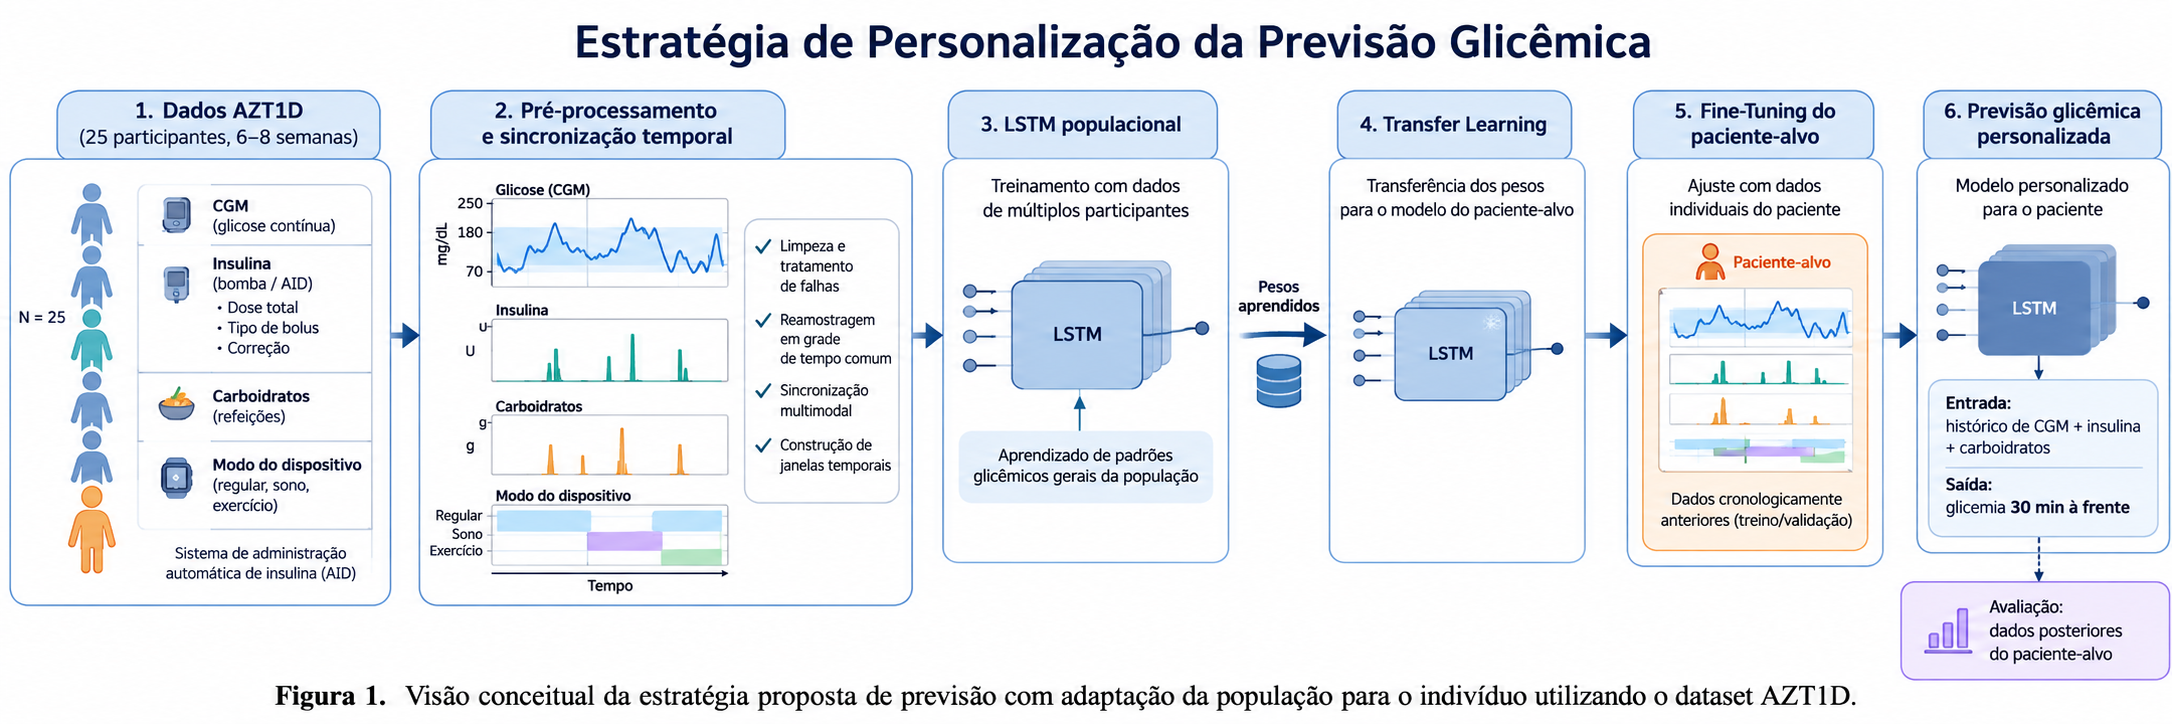
\includegraphics[width=0.55\textwidth]{bace593d-4823-4a49-8768-bc1016f0c5fc.png}
    \caption{Visão conceitual da estratégia proposta de previsão com adaptação
da população para o indivíduo.}
\end{figure}

\section{Materiais e Métodos}
\label{sec:materiais}

O conjunto de dados selecionado é o AZT1D, disponibilizado no Mendeley Data sob o DOI 10.17632/gk9m674wcx.1 e licença CC BY 4.0~\cite{azt1d_dataset}. A base contém dados reais de 25 indivíduos com DM1, coletados durante aproximadamente 6--8 semanas por participante, incluindo CGM, administração de insulina, ingestão de carboidratos e modos do dispositivo~\cite{azt1d_dataset}. O conjunto possui aproximadamente 320 mil registros de CGM e mais de 26 mil horas de monitoramento, oferecendo histórico longitudinal adequado para o treinamento populacional e posterior personalização~\cite{khamesian2026glimmer}.

A entrada preditiva inicial combinará \textbf{CGM, insulina e carboidratos}, enquanto o modo do dispositivo poderá ser incorporado posteriormente como variável adicional. Entradas multivariadas podem contribuir para modelos de previsão glicêmica, embora seu benefício dependa da abordagem utilizada~\cite{nemat2024comparative}. Como configuração inicial, aproximadamente 60 minutos de dados históricos serão utilizados para prever a glicemia 30 minutos à frente.

O modelo principal será uma rede neural recorrente Long Short-Term Memory (LSTM) compacta~\cite{hochreiter1997lstm}, arquitetura amplamente utilizada em previsão de séries temporais glicêmicas~\cite{khadem2026ai}. Os registros de CGM, insulina e carboidratos serão alinhados temporalmente, com tratamento de valores ausentes e normalização calculada exclusivamente sobre os dados de treinamento.

O desenho experimental separará os participantes em nível de indivíduo para evitar vazamento de dados. A LSTM será inicialmente treinada com um grupo populacional, enquanto participantes separados permanecerão não observados nessa etapa. Para cada participante-alvo, uma parte cronologicamente anterior dos dados será utilizada para fine-tuning e uma parte posterior para avaliação. Serão comparados o modelo populacional sem adaptação e o mesmo modelo após transfer learning e fine-tuning. Caso seja viável, também será incluído um modelo treinado do zero apenas com dados individuais e serão testadas diferentes quantidades de dados para personalização.

O fine-tuning utilizará os pesos aprendidos pelo modelo populacional e uma taxa de aprendizado reduzida. Estratégias semelhantes de transferência de conhecimento já foram investigadas em previsão glicêmica personalizada e em outros sinais fisiológicos~\cite{deng2021transfer,shen2025incremental,leitner2022bp}. Como experimento adicional, poderá ser comparado o fine-tuning de toda a rede com a atualização apenas das camadas finais.

O desempenho será avaliado principalmente por Root Mean Squared Error (RMSE) e Mean Absolute Error (MAE), com resultados apresentados por participante e de forma agregada. Caso seja viável, a Clarke Error Grid será utilizada como análise clínica complementar~\cite{clarke1987errorgrid}. A implementação será realizada em Python utilizando TensorFlow/Keras, NumPy, pandas, scikit-learn e Matplotlib, com execução no Google Colab e em computadores locais.


\begin{figure}[!htp]
\centering

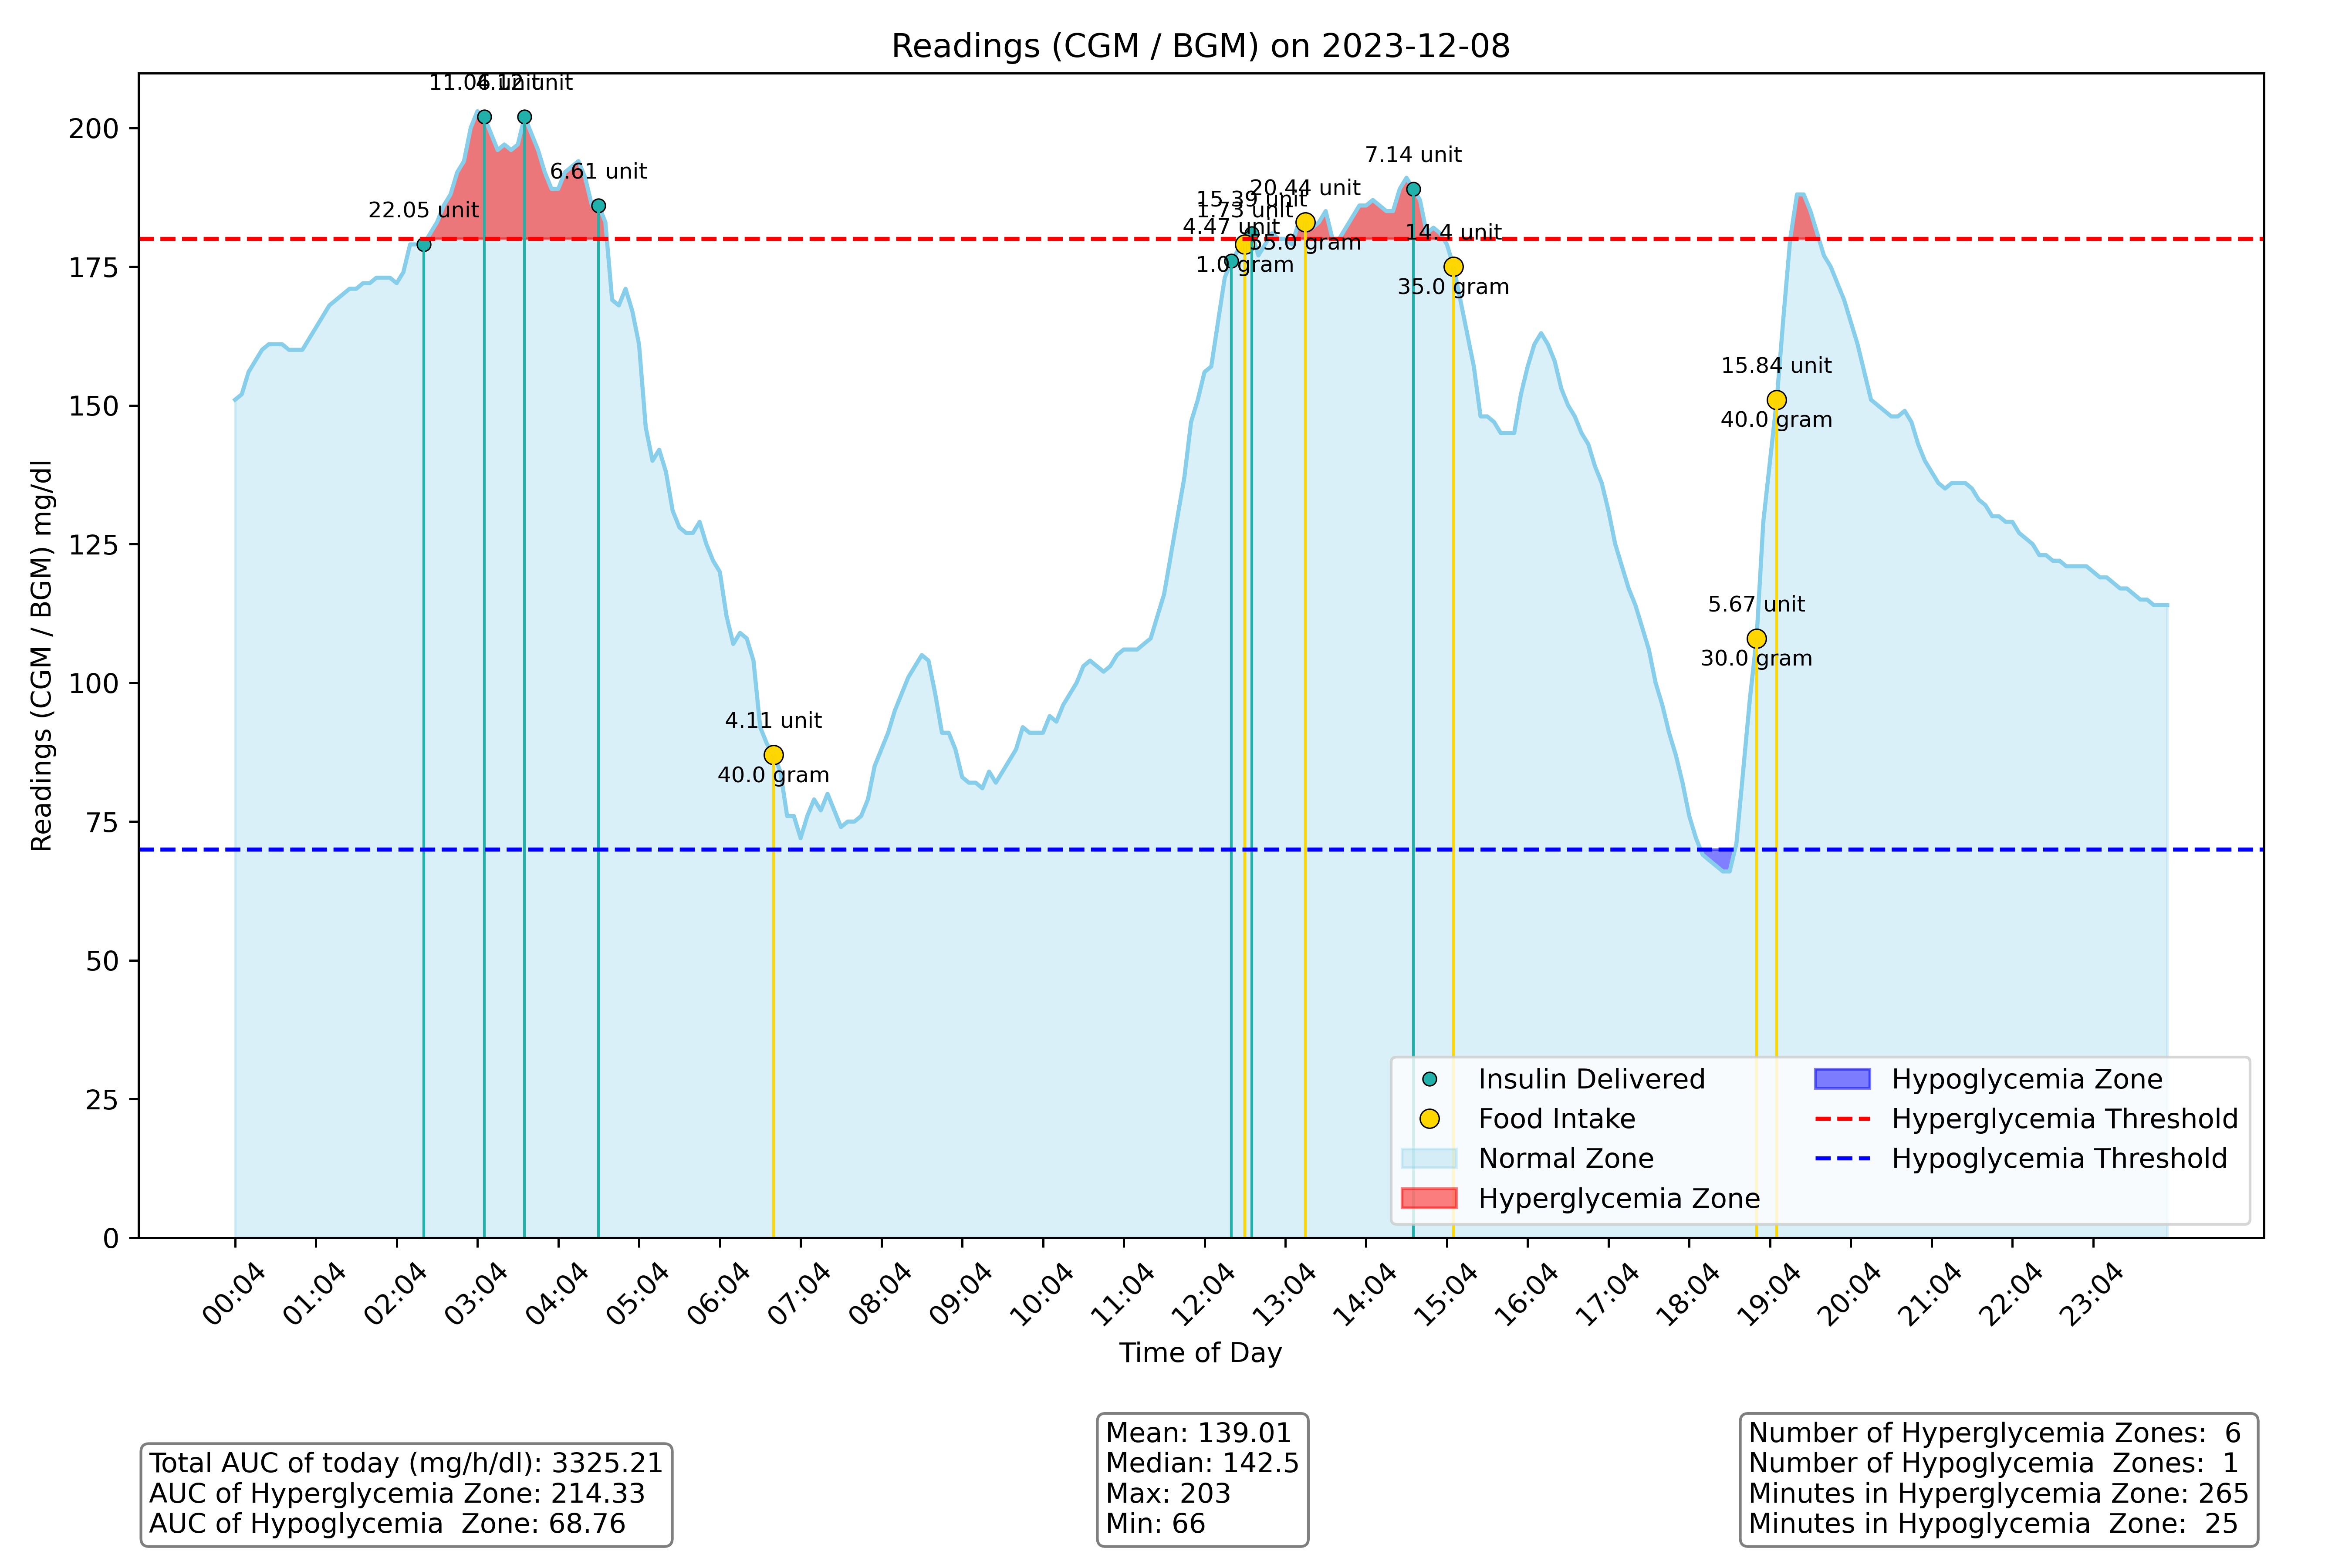
\includegraphics[width=0.48\columnwidth]{Readings_2023-12-08.png}
\hfill
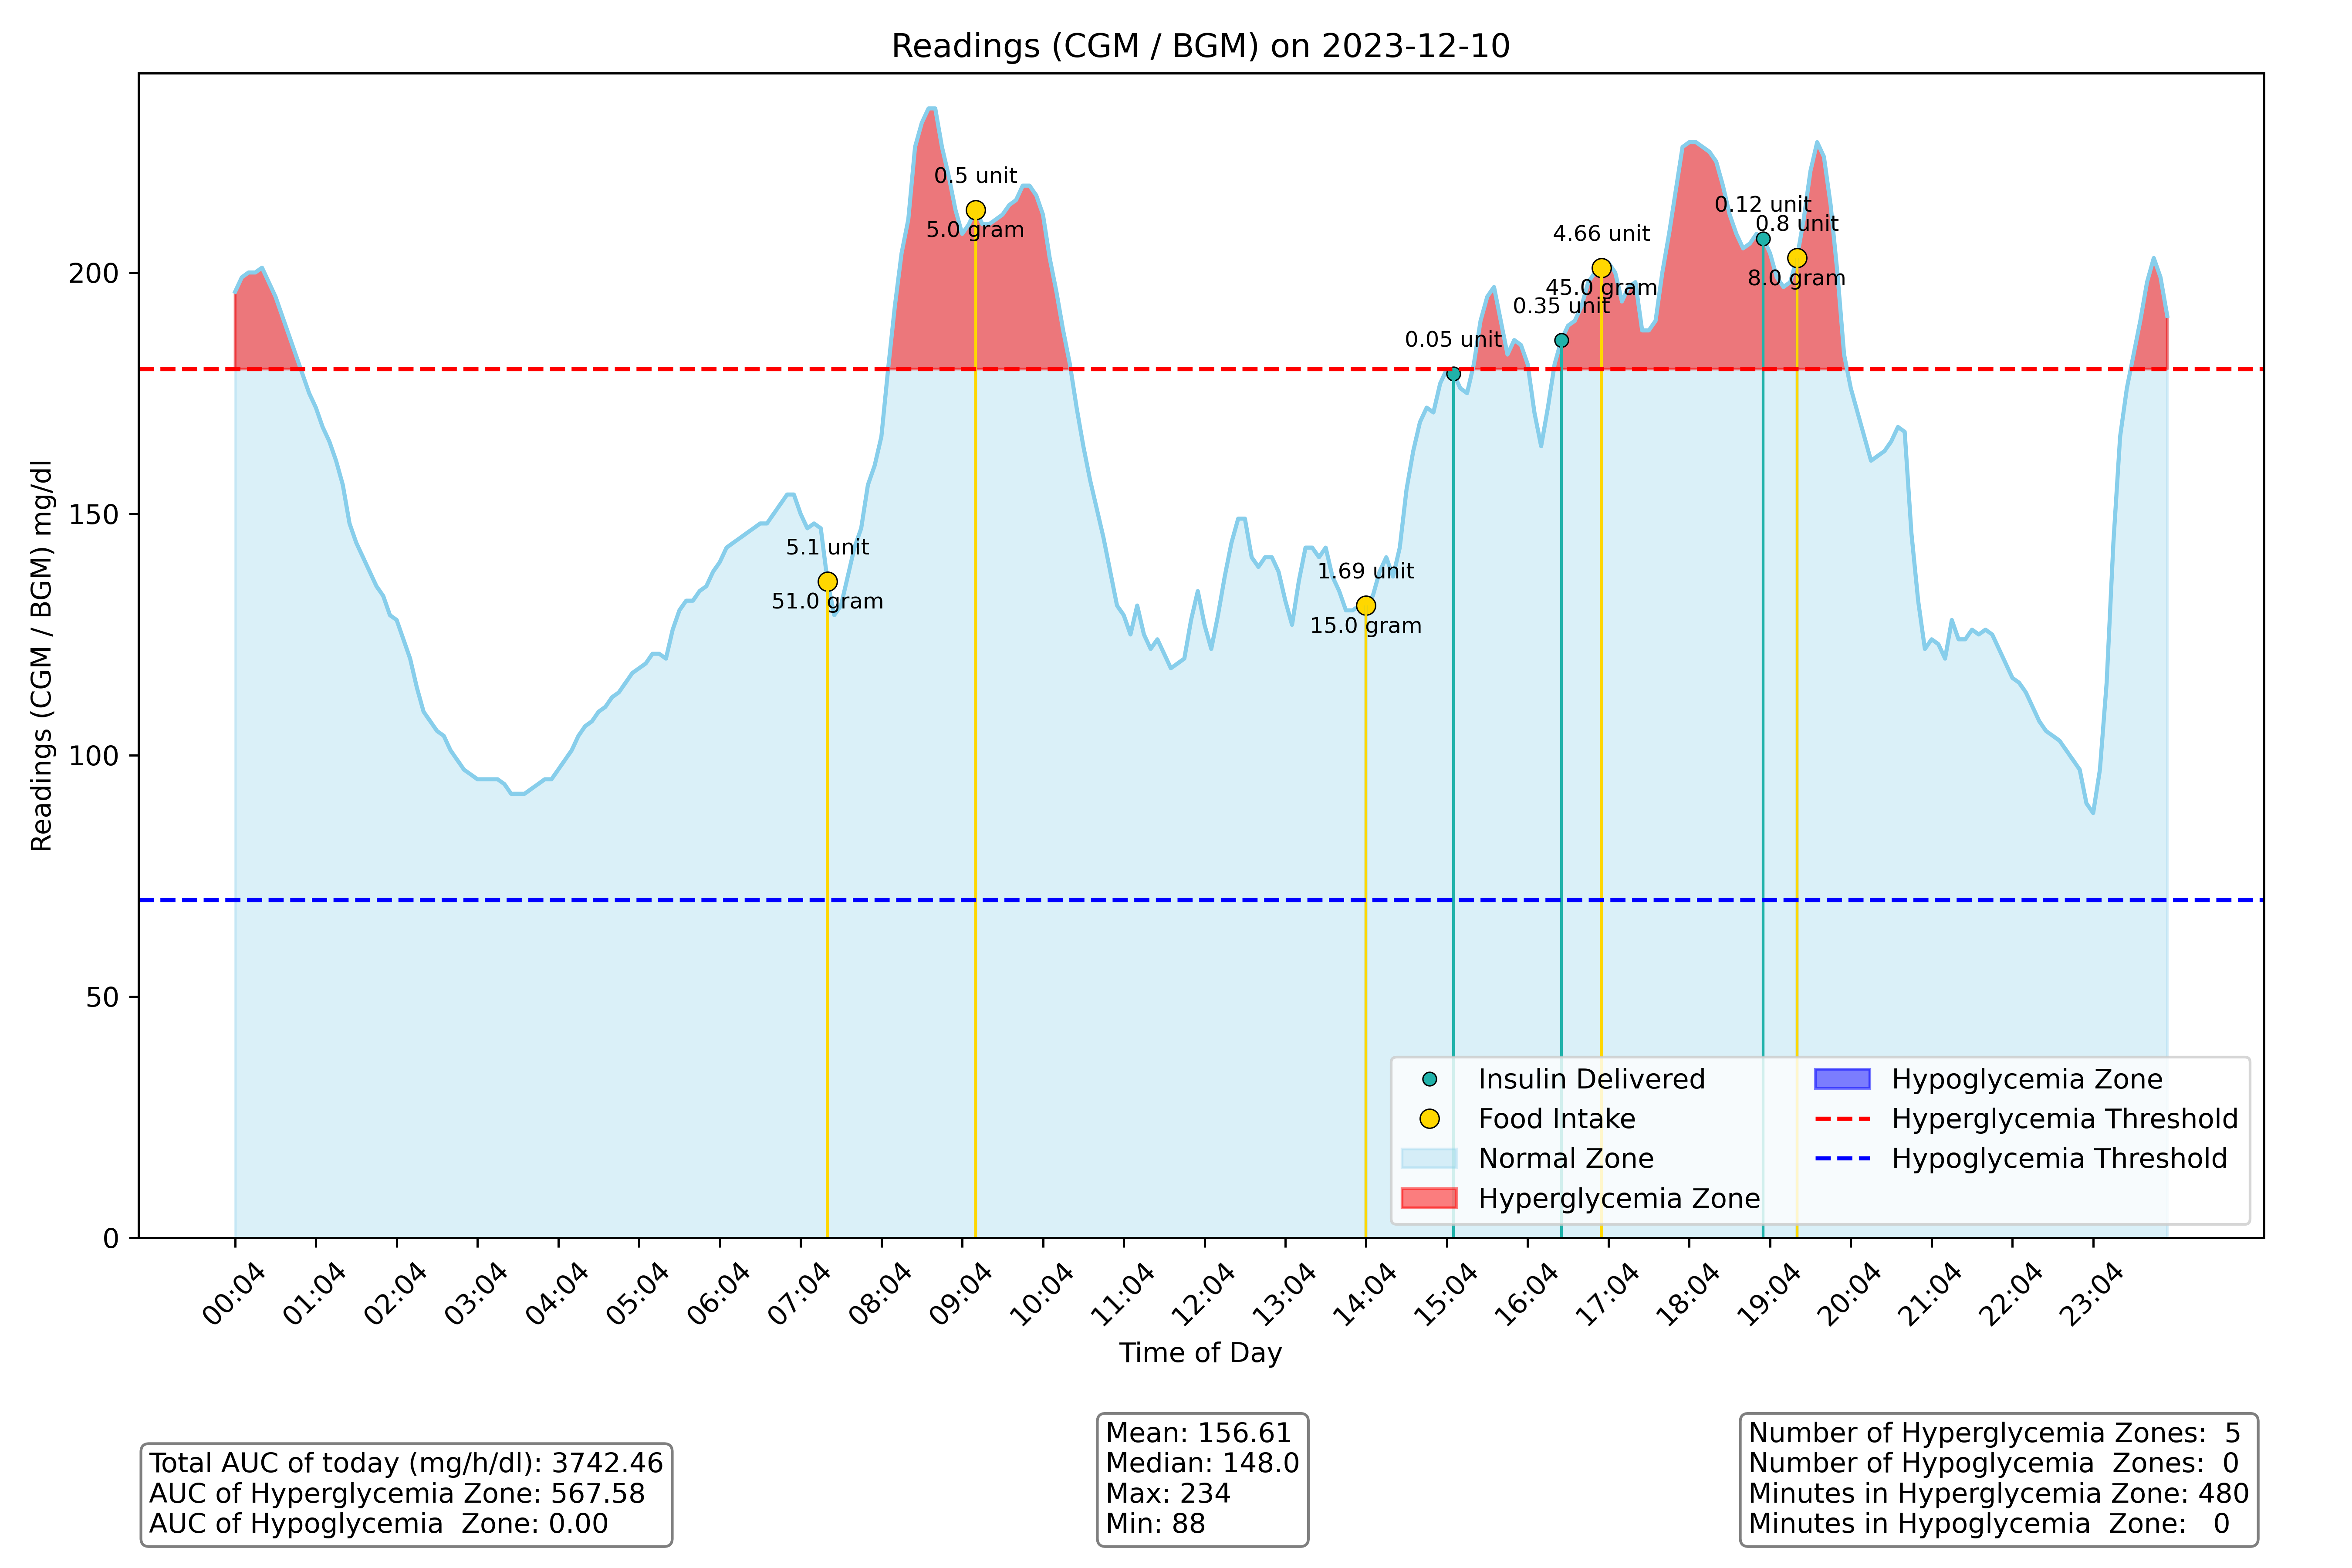
\includegraphics[width=0.48\columnwidth]{Readings_2023-12-10.png}

\caption{Comparação de glucose, insulina e leitura de carboidratos para o Subject 1 e o Subject 2}
\label{fig:subjects_comparison}
\end{figure}

\begin{table*}[!htp]
\centering
\renewcommand{\arraystretch}{1.4} % increases row spacing

\caption{Resumo de Materiais e Métodos.}
\label{tab:materiais_metodos2}

\vspace{-1.5mm} % reduces space between caption and table

% adjusts table width to text width
\resizebox{0.95\textwidth}{!}{%
\begin{tabular}{|p{3cm}|p{7cm}|p{6cm}|}
\hline
\textbf{Materiais} & \textbf{Descrição} & \textbf{Observações} \\
\hline

Conjunto de dados & AZT1D~\cite{azt1d_dataset,khamesian2026glimmer} & Dados reais de 25 indivíduos com DM1, contendo CGM, insulina, carboidratos e modos do dispositivo durante aproximadamente 6--8 semanas por participante. \\
\hline
Modelos & LSTM populacional e LSTM personalizada por fine-tuning~\cite{hochreiter1997lstm} & Mesma arquitetura antes e depois da personalização. \\
\hline
Técnicas & Transfer Learning, Fine-Tuning e Fine-Tuning Parcial opcional & Estratégia de personalização selecionada~\cite{deng2021transfer,shen2025incremental,leitner2022bp}. \\
\hline
Linguagens / Bibliotecas & Python, TensorFlow/Keras, NumPy, pandas, scikit-learn, Matplotlib & Ambiente principal de aprendizado de máquina e pré-processamento. \\
\hline
Hardware / Recursos & Google Colab e computadores locais disponíveis & Espera-se que seja suficiente para os experimentos repetidos de treinamento e fine-tuning. \\
\hline
Outros Recursos & Mendeley Data, Git/GitHub & Download do conjunto e pacote de reprodutibilidade. \\
\hline
Entradas / Saída & CGM + insulina + carboidratos; glicemia 30 min à frente & Modo do dispositivo reservado como entrada adicional opcional. \\
\hline
Avaliação & RMSE, MAE e grade de erro clínico opcional & Comparação entre modelo populacional, modelo com fine-tuning e modelo opcional treinado do zero. \\
\hline
\end{tabular}%
}
\end{table*}


\section{Etapas do Projeto e Marcos Físicos}
\label{sec:etapas}

Etapa 1 -- Revisão do estado da arte e definição do protocolo.
Consolidar referências sobre DM1, CGM, previsão glicêmica, variabilidade entre pacientes, transfer learning e fine-tuning. Confirmar a pergunta de pesquisa final, variáveis de entrada, horizonte de previsão, divisão dos participantes e métricas de avaliação.
\textit{Marco:} protocolo experimental e bibliografia finalizados.

Etapa 2 -- Aquisição e pré-processamento do AZT1D.
Baixar o conjunto de dados pelo Mendeley Data, inspecionar arquivos e identificadores, alinhar registros de CGM, insulina e carboidratos, tratar valores ausentes, criar janelas temporais e definir os grupos de treinamento, validação e participantes-alvo.
\textit{Marco:} pipeline de pré-processamento reproduzível e divisão do conjunto documentada.

Etapa 3 -- Baseline LSTM populacional.
Implementar a LSTM multivariada, treiná-la utilizando apenas os participantes do conjunto populacional, ajustar os hiperparâmetros essenciais e estabelecer valores de RMSE/MAE em participantes não observados antes da personalização.
\textit{Marco:} pesos salvos do modelo populacional, código-fonte, log de execução e resultados de baseline.

Etapa 4 -- Transfer learning e fine-tuning específico por paciente.
Carregar os pesos populacionais para cada participante-alvo e realizar o fine-tuning utilizando uma parte cronologicamente anterior dos dados desse participante. Preservar os dados posteriores exclusivamente para avaliação.
\textit{Marco:} pipeline funcional de treinamento personalizado e primeira comparação entre modelo populacional e personalizado.

Etapa 5 -- Experimentos de personalização.
Repetir o fine-tuning utilizando diferentes quantidades de dados individuais e, se viável, comparar fine-tuning completo, fine-tuning parcial e treinamento do zero. Repetir o protocolo em múltiplos participantes-alvo.
\textit{Marco:} tabelas e gráficos apresentando erro por participante, estratégia e quantidade de dados pessoais.

Etapa 6 -- Análise dos resultados.
Agregar RMSE/MAE, analisar indivíduos com altos e baixos ganhos de personalização, avaliar a influência da variabilidade entre pacientes e discutir limitações relacionadas a eventos autorrelatados, dados ausentes, exercício e composição do conjunto.
\textit{Marco:} figuras experimentais finais, tabelas e notas para discussão.

Etapa 7 -- Manuscrito e pacote de reprodutibilidade.
Consolidar o artigo e organizar o repositório com scripts de pré-processamento, código do modelo, configuração dos experimentos, logs, resultados e instruções de execução.
\textit{Marco:} manuscrito pronto para submissão e repositório reproduzível.

\section{Cronograma}
\label{sec:cronograma}

\begin{table}[!htp]
\centering
\renewcommand{\arraystretch}{1.3}
\caption{Cronograma do projeto considerando as datas oficiais das Entregas 02 e 03a.}
\label{tab:cronograma}

\vspace{-1.5mm}

\resizebox{0.99\linewidth}{!}{%
\begin{tabular}{l c c c c c c}
\toprule
\textbf{Atividade} &
\makecell[c]{\textbf{29/08--11/09}} &
\makecell[c]{\textbf{12/09--25/09}} &
\makecell[c]{\textbf{26/09--09/10}} &
\makecell[c]{\textbf{10/10--23/10}} &
\makecell[c]{\textbf{24/10--31/10}} &
\makecell[c]{\textbf{01/11--09/11}} \\
\midrule
\rowcolor{gray!10} Levantamento do estado da arte & \cmark & \cmark &   &   &   &   \\
Processamento AZT1D                         & \cmark & \cmark & \cmark &   &   &   \\
\rowcolor{gray!10} LSTM populacional       &        & \cmark & \cmark & \cmark &   &   \\
Transfer learning / fine-tuning             &        &        & \cmark & \cmark & \cmark &   \\
\rowcolor{gray!10} Experimentação / resultados &   &        &        & \cmark & \cmark &   \\
Escrita do artigo                           &  &  &  & \cmark & \cmark & \cmark \\
\rowcolor{gray!10} Pôster                  &        &        &        &        & \cmark & \cmark \\
\bottomrule
\end{tabular}%
}
\end{table}


\bibliographystyle{IEEEtran}
\bibliography{bibtex}



\end{document}